\begin{figure*}
  \centering
    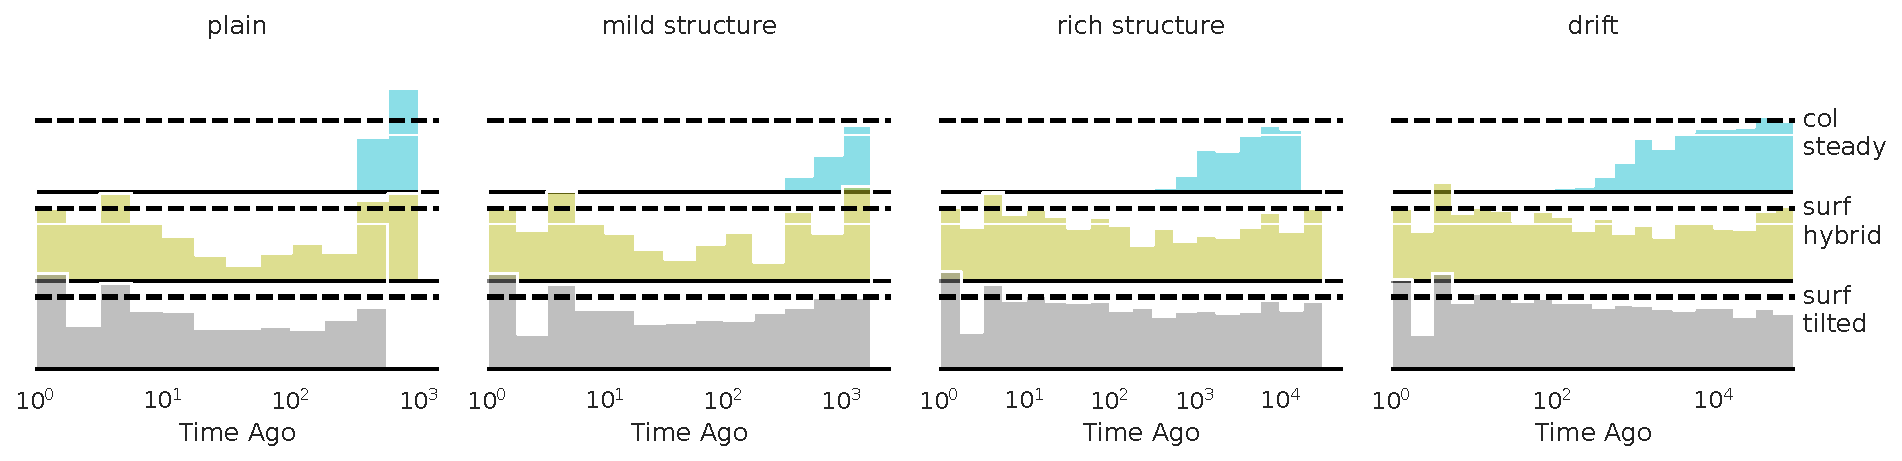
\includegraphics[width=\linewidth]{binder/binder/teeplots/annotation-size=256+col=scenario+differentia-width=8+hue=kind+row=algo+scale=npop65536-ngen100000+viz=joyhist+x=time-ago+ext=}
\caption{%
\textbf{How does retention policy affect the structure of inner node loss?}
Reconstruction node count densities for 256-bit size, byte differentia treatments.
Histograms depict internal node count relative to reference trees (dashed line), binned by time ago (ranging from most recent to most ancient).
Facet columns differentiate evolutionary regimes and facet rows correspond to steady, hybrid, and tilted retention policies.
Owing to its non-prioritization to retain recent differentiae, steady policy loses nearly all resolution over recent (c. 100 generations) evolutionary history.
Tilted policy, on the other hand, reconstructs the highest proportion of recent history.
Hybrid policy does not suffer the catastrophic inner node loss over recent events seen under steady policy, but also reconstructs somewhat fewer recent inner nodes compared to pure tilted policy.
}
  \label{fig:recency-structure}

\end{figure*}
